\documentclass[tikz]{standalone}

\begin{document}
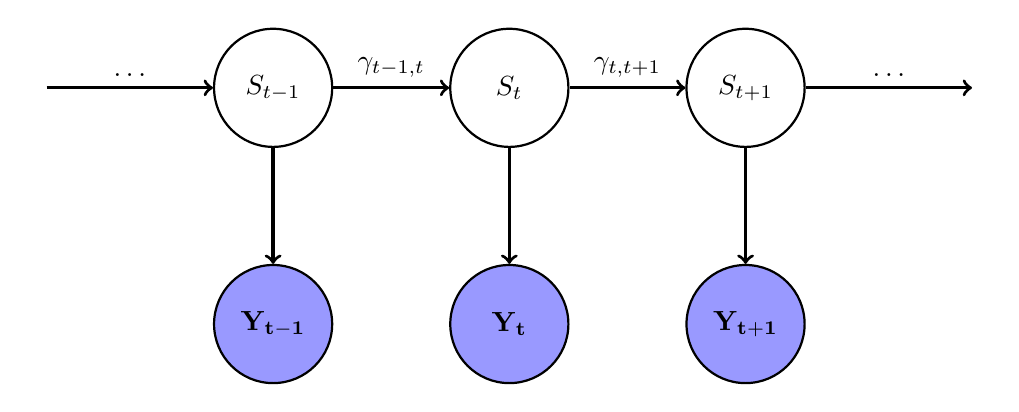
\begin{tikzpicture}[node distance=3cm]

% Define the node styles
\tikzstyle{state}=[circle, draw, thick, minimum size=1.5cm, align=center]
\tikzstyle{observation}=[circle, draw, thick, fill=blue!40, minimum size=1.5cm, align=center]
% Define the nodes
\node[yshift=-1cm] (beginning) {};
\node[state, right of = beginning] (state1) {$S_{t-1}$};
\node[state, right of=state1] (state2) {$S_{t}$};
\node[state, right of=state2] (state3) {$S_{t+1}$};
\node[observation, below of=state1] (obs1) {$\mathbf{Y_{t-1}}$};
\node[observation, below of=state2] (obs2) {$\mathbf{Y_{t}}$};
\node[observation, below of=state3] (obs3) {$\mathbf{Y_{t+1}}$};
\node[right of=state3] (end) {};

% Add the edges
\path[->, very thick] (beginning)  edge[] node[midway, above] {$\dots$} (state1)
          (state1) edge[] node[midway, above] {$\gamma_{t-1,t}$} (state2)
          (state2) edge[] node[midway, above] {$\gamma_{t,t+1}$} (state3)
          (state1) edge node[midway, left] {} (obs1)
          (state2) edge node[midway, left] {} (obs2)
          (state3) edge node[midway, right] {} (obs3)
          (state3) edge[] node[midway, above] {$\dots$} (end);

\end{tikzpicture}
\end{document}